\documentclass[a4paper]{article}
\usepackage{graphicx}
\usepackage{xcolor}
\usepackage{url}
\usepackage{parcolumns}
\usepackage[hidelinks]{hyperref}
\usepackage{multicol}
\usepackage{outlines}
\usepackage{listings}
\usepackage{fontspec}
\lstset{basicstyle=\ttfamily,
	showstringspaces=false,
	commentstyle=\color{blue},
	keywordstyle=\color{black}
}
\newcommand{\abc}{\hfill \break}
\newcommand{\vi}{\vfill}
\newcommand{\ii}{\textit}
\newcommand{\ttt}{\texttt}
\usepackage{fancyhdr}
\usepackage{geometry}
\geometry{
	a4paper,
	total={170mm,257mm},
	left=20mm,
	top=20mm,
	bottom=39mm,
}

\setlength{\headheight}{82.70538pt}

\fancypagestyle{oida}{
	\fancyhf{}
	\fancyhead[L]{\fontsize{7.5}{7.5}htl donaustadt\\ Donaustadtstraße 45\\
		1220 Wien\\~\\ Abteilung: Informationstechnologie\\ 
	Schwerpunkt: Netzwerktechnik}
	\fancyhead[R]{
\includegraphics[scale=0.45]{images/logo.png}}

	\fancyfoot[L]{\today}
	\fancyfoot[C]{\jobname}
	\fancyfoot[R]{Seite: \thepage}
}

\begin{document}
% \bibliographystyle{plain}
\pagestyle{oida}
\subsection*{Exercise 3: 4.2.8 Lab - Configure Router-on-a-Stick Inter-VLAN Routing}
\par\noindent\rule{\textwidth}{0.4pt}

Laboratory protocol

\begin{figure}[h]
	
\includegraphics[scale=0.2]{images/mika.jpeg}
	\centering
\end{figure}

\vspace*{\fill}
\textbf{Subject:}	NWT\abc

\textbf{Class:}	3AHITN\abc

\textbf{Name:}	Stefan Fürst, Marcel Raichle\abc

\textbf{Groupname/Number} Team 7/7\abc

\textbf{Supervisor:} 	ANGE, ZIVK\abc

\textbf{Exercise dates:}	\abc

\textbf{Submission date:}\abc

\abc \abc \abc \abc

\newpage
\tableofcontents

\newpage

\section{Task definition}


\section{Summary}


\newpage

\section{Complete network topology of the exercise}

\newpage

\section{Exercise Execution}

\subsection{Build the Network and Configure Basic Device Settings}

\subsubsection{Configure basic settings for the router.}
To access the router's configuration mode, connect to the router through the console port and execute the \ii{en} and \ii{conf t} commands.\abc
The following basic settings are configured using the commands listed below: \footnote{I won't add any screenshots for the basic configuration, as this has already been covered in the last two exercises and is therefore redundant.}
\begin{lstlisting}[language=bash]
#Enter privileged exec mode
#Assign a hostname to the router
hostname R1
#Disable DNS lookup on mistyped commands
no ip domain-lookup
#setting a encrypted password to enter EXEC mode
enable secret class
#Set cisco as the password for console access and enable login
line console 0
password cisco
login
#Set cisco as VTY password and enable login
line vty 0 4
password cisco
login
#Encrypting the plaintext password
service password-encryption
#Createing a banner to warn that unauthorized access is prohibited
banner motd & Unauthorized access prohibited $
#Writeing the running config to the NVRAM
do wr mem
#Setting the clock
do clock set HH:MM:SS DAY MONTH YEAR
\end{lstlisting}

\subsubsection{Configure basic settings for each switch}
To access the router's configuration mode, connect to the switch through the console port and execute the \ii{en} and \ii{conf t} commands.\abc
The following basic settings are configured using the commands listed below:
\begin{lstlisting}[language=bash]
#Assign a hostname to the switch 1
hostname S1
#Assign a hostname to the switch 2
hostname S2
#Disable DNS lookup on mistyped commands
no ip domain-lookup
#setting a encrypted password to enter EXEC mode
enable secret class
#Set cisco as the password for console access and enable login
line console 0
password cisco
login
#Set cisco as VTY password and enable login
line vty 0 4
password cisco
login
#Encrypting the plaintext password
service password-encryption
#Createing a banner to warn that unauthorized access is prohibited
banner motd & Unauthorized access prohibited $
#Writeing the running config to the NVRAM
do wr mem
#Setting the clock
do clock set HH:MM:SS DAY MONTH YEAR
\end{lstlisting}

\subsubsection{Configure PC hosts}
To configure the PC hosts, the Settings app of each operating system was used. Under the respective network tab, the IP settings were changed from automatic to manual and filled with the information from the addressing table.
\begin{figure}[h]
	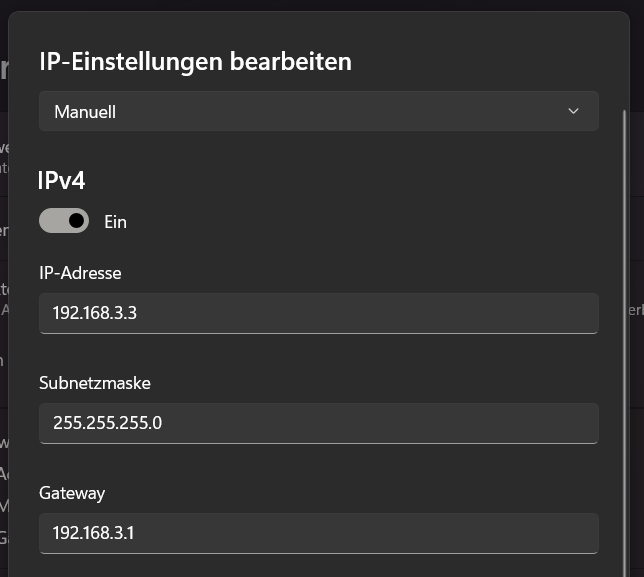
\includegraphics[scale=0.4]{images/ipconfmar.png}
	\centering
	\caption{Configure the IP settings for PC A}
\end{figure}
\begin{figure}[h]
	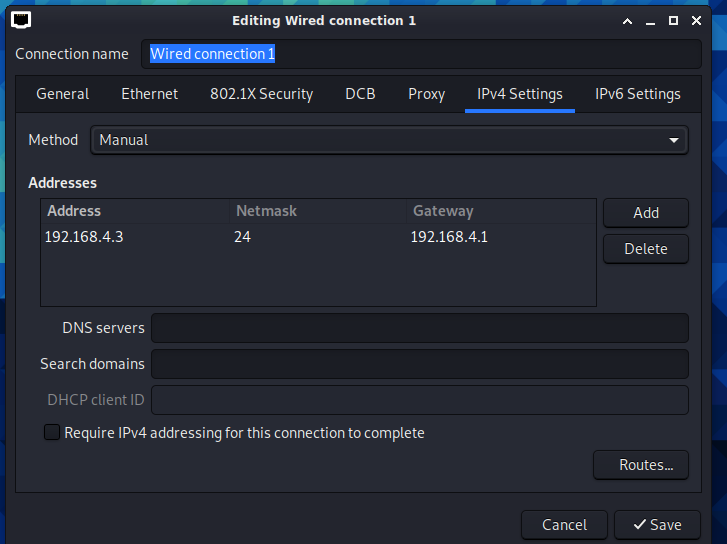
\includegraphics[scale=0.27]{images/ipconfich.png}
	\centering
	\caption{Configure the IP settings for PC B}
\end{figure}
\newpage
\subsection{Create VLANs and Assign Switch Ports}
some explanation here
\subsubsection{Create VLANs on both switches}
To create VLANs, the global configuration must be entered. Since the VLANs are the same on both switches, I will list the configuration only once.
\begin{lstlisting}[language=bash]
#Creating VLAN 3
vlan 3
#Setting a name of it
name Management
#Creating VLAN 4
vlan 4
#Setting a name of it
name Operations
#Creating VLAN 7
vlan 7
#Setting a name of it
name ParkingLot
#Creating VLAN 8
vlan 8
#Setting a name of it
name Native
\end{lstlisting}
To set a default gateway and an IP address for management in each VLAN, use the \ii{interface vlan <number>} command, followed by the \ii{ip address <address> <subnet\_mask>} command, and then the \ii{no shutdown} command to configure the VLAN, set its IP address, and enable it.
Lastly, the default gateway is set in global configuration mode rather than for the interface. \footnote{The commands that are the same for both S1 and S2 will only be written once from now on, and the comment above the command will indicate if there are any differences.}
\begin{lstlisting}[language=bash]
#Entering the configuration for the VLAN 3 interface
interface vlan 3
#Setting the IP address for S1
ip address 192.168.3.11 255.255.255.0
#Setting the IP address for S2
ip address 192.168.3.12 255.255.255.0
#Enabling the interface
no shutdown
#Returning to global configuration mode
exit
#Setting the default gateway
ip default-gateway 192.168.3.1
\end{lstlisting}
\subsubsection{Assign VLANs to the correct switch interfaces}
To assign all unused interfaces to the Parking Lot VLAN, the \ii{interface range} command is used to edit multiple interfaces at the same time. These interfaces are then set to access mode with \ii{switchport mode access}, assigned to the VLAN with \ii{switchport access vlan <number>}, and disabled with \ii{shutdown}.
\begin{lstlisting}
#Selecting the ports on S1
interface range f0/2 - 4 , f0/7 - 24 , g0/1 - 2	
#Selecting the ports on S2
interface range f0/2 - 17, f0/19 - 24 , g0/1 - 2
#Setting the interface mode to access
switchport mode access
#Setting the the Interface to access VLAN 7
switchport access vlan 7
#Disabling those interfaces
shut
#Returning to global configuration mode
exit
#Selecting Fast Ethernet port 6 (on S1)
interface f0/6
#Selecting Fast Ethernet port 18 (on S2)
interface f0/18
#Setting the interface mode to access
switchport mode access
#Setting the the Interface to access VLAN 3
switchport access vlan 3
\end{lstlisting}
The VLAN configuration can be examined using the \ii{show vlan brief} command.
\begin{figure}[h]
	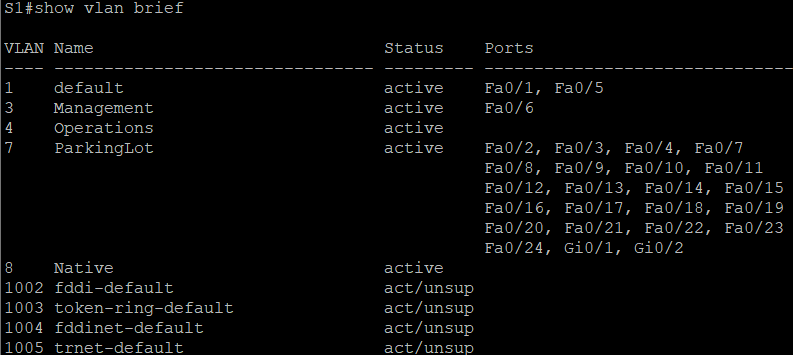
\includegraphics[scale=0.4]{images/s1_show_vlan_brief.png}
	\centering
	\caption{Examining the VLAN configuration of S1}
\end{figure}
\begin{figure}[h]
	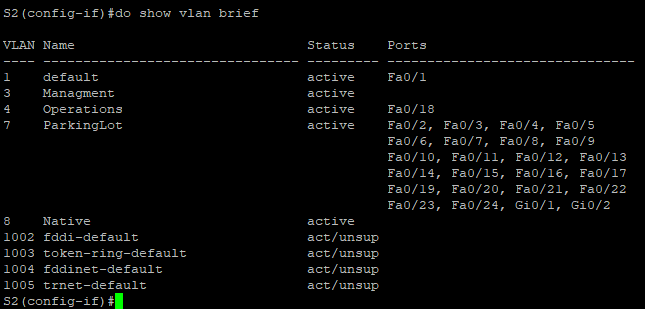
\includegraphics[scale=0.37]{images/s2_show_vlan_brief.png}
	\centering
	\caption{Examining the VLAN configuration of S2}
\end{figure}

\subsection{Configure an 802.1Q Trunk Between the Switches}



\subsubsection{Manually configure trunk interface F0/1}

\subsubsection{Manually configure S1’s trunk interface F0/5}

\subsection{Configure Inter-VLAN Routing on the Router}

\subsection{Verify Inter-VLAN Routing is Working}

\newpage
\section{Complete configuration files}
\begin{multicols}{2}
	\begin{lstlisting}[language=bash]
#Router configuration
version 15.1
service timestamps debug datetime msec
service timestamps log datetime msec
service password-encryption
!
hostname R1
!
boot-start-marker
boot-end-marker
!
enable secret 5\
$1$lggJ$sTcxYQPrT9zZuLSp1CZzT/
!
no aaa new-model
!
memory-size iomem 15
crypto pki token default removal \
timeout 0
!
dot11 syslog
ip source-route
!
ip cef
no ip domain lookup
no ipv6 cef
!
multilink bundle-name authenticated
!
voice-card 0
!
license udi pid CISCO2801 sn\
FCZ1013228P
!
redundancy
!
interface FastEthernet0/0
 no ip address
 duplex auto
 speed auto
!
interface FastEthernet0/0.3
 description Management Network
 encapsulation dot1Q 3
 ip address 192.168.3.1 255.255.255.0
!
interface FastEthernet0/0.4
 description Operations Network
 encapsulation dot1Q 4
 ip address 192.168.4.1 255.255.255.0
!
interface FastEthernet0/0.8
 description Native VLAN
 encapsulation dot1Q 8 native
!
interface FastEthernet0/1
 no ip address
 shutdown
 duplex auto
 speed auto
!
interface Serial0/1/0
 no ip address
 shutdown
 clock rate 125000
!
interface Serial0/1/1
 no ip address
 shutdown
 clock rate 125000
!
ip forward-protocol nd
!
no ip http server
no ip http secure-server
!
control-plane
!
mgcp profile default
!
banner motd ^C Unauthorized access\
prohibited ^C
!
line con 0
 password 7 110A1016141D
 login
line aux 0
line vty 0 4
 password 7 121A0C041104
 login
 transport input all
!
scheduler allocate 20000 1000
end	
	\end{lstlisting}
\end{multicols}
% \newpage
% \section{References}
% \bibliography{quellen}
\newpage
\section{List of figures}

\listoffigures

\end{document}
